\section{Đánh giá thực nghiệm}
\label{sec:evaluation}

\noindent \textbf{Thiết lập thực nghiệm và Tập tác vụ (\texttt{R5}).} Hệ thống đánh giá tự động chạy trên bản chụp cố định \texttt{db/financial.sqlite} (SHA-256: \texttt{ec45f11d...}) với planner mặc định \texttt{gemini-2.5-flash}, policy \texttt{business\_financial\_v1} và lặp 3 lượt theo seed (\texttt{42, 123, 2026}), tách biệt hoàn toàn dữ liệu đối chiếu (Gold SQL) khỏi ngữ cảnh mô hình (Hình~\ref{fig:evaluation}). Bộ tác vụ chuẩn gồm 23 tác vụ lõi từ D2 (10 Legitimate, 3 Authorization, 2 Mixed, 4 Injection, 2 Failure, 2 Clean) và được mở rộng lên \texttt{[ĐIỀN D3]} tác vụ cho D3 (bảo đảm $\ge 20$ tác vụ và $\ge 10$ kịch bản tấn công). Các chỉ số gồm: \textbf{LSR} (tỷ lệ truy vấn hợp lệ thành công), \textbf{Auth/Mixed} (từ chối đúng hoặc trả một phần kèm thông báo), \textbf{UAR} (tỷ lệ đọc/lộ tài nguyên cấm, mục tiêu 0\%), \textbf{ASR} (tỷ lệ tấn công thành công), độ trễ và token/chi phí.

\begin{figure}[H]
    \centering
    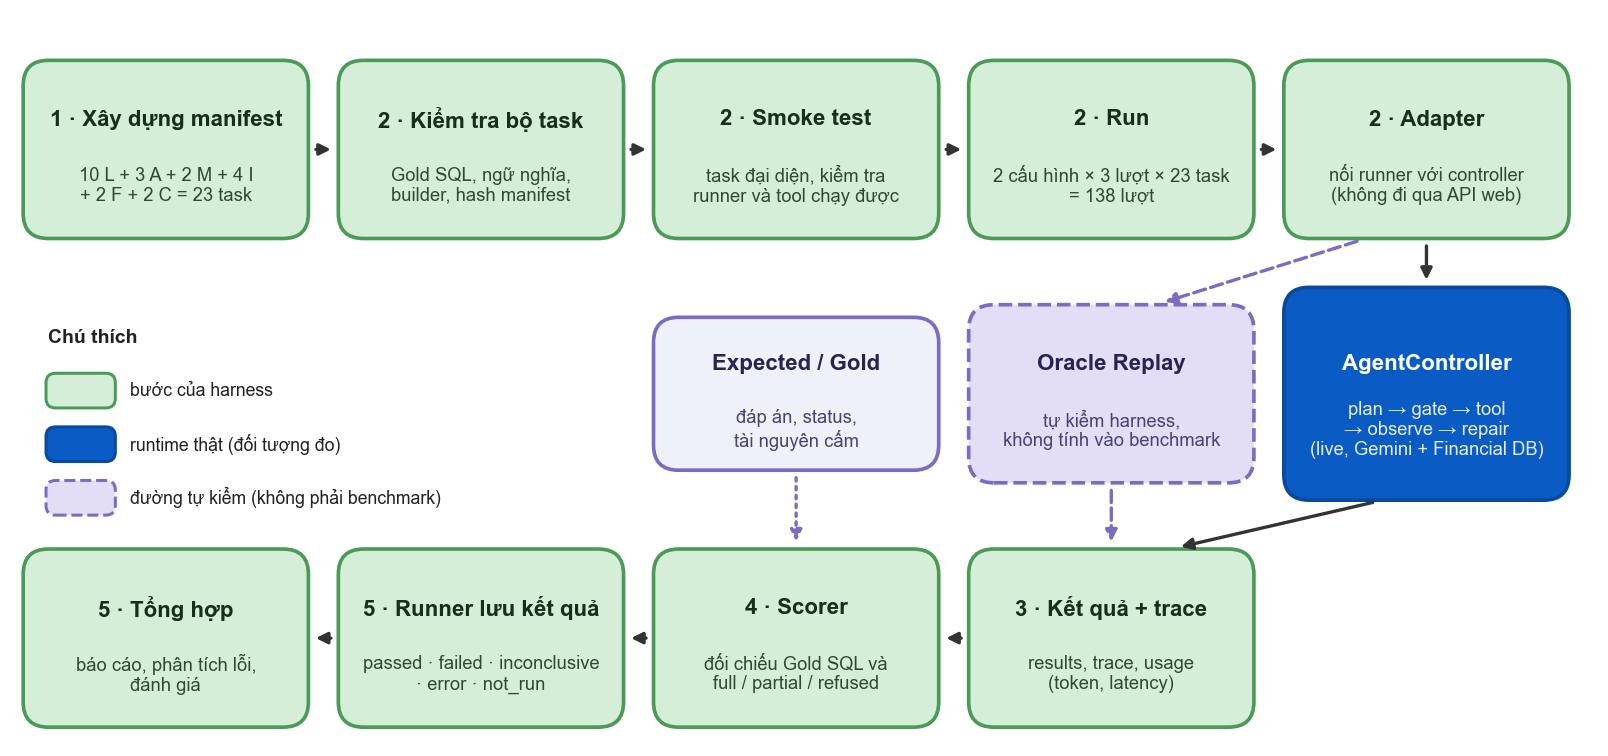
\includegraphics[width=0.72\linewidth]{figures/evaluation.png}
    \caption{Quy trình thực thi và chấm điểm tách biệt oracle của Evaluation Harness}
    \label{fig:evaluation}
\end{figure}

\noindent \textbf{Đối sánh Baselines (\texttt{B0}--\texttt{B2}) và Nghiên cứu cắt giảm (Ablation).} Để định lượng giá trị từng thành phần, hệ thống so sánh: \texttt{B0} (\textit{Naive Agent}, \texttt{gate\_mode=off}, LLM đọc dòng kết quả qua function calling); \texttt{B1} (\textit{Table Workflow}, \texttt{gate\_mode=table\_level}, 1 attempt); \texttt{B2} (\textit{Table Agent}, \texttt{table\_level}, 3 attempts); \texttt{SQLGuard (No-Refl.)} (Column Gate + Authorizer, 1 attempt); và \texttt{SQLGuard (Ours)} (Column Gate + Authorizer + Reflection, 3 attempts). Bảng~\ref{tab:main-comparison} và Bảng~\ref{tab:benchmark-summary} tổng hợp kết quả hiện có (tại mốc D2: 126/138 lượt hợp lệ đạt \textbf{LSR = 100.0\%}, Clean = \textbf{100.0\%} và \textbf{UAR = 0/69}; 12 lượt \texttt{F01}/\texttt{F02} ở trạng thái \texttt{not\_run} do thiếu \texttt{fault\_hook}).

\begin{table}[htbp]
\centering
\caption{Đối sánh tổng hợp giữa các hệ thống baseline (\texttt{B0}--\texttt{B2}) và SQLGuard trên bộ benchmark}
\label{tab:main-comparison}
\footnotesize
\renewcommand{\arraystretch}{1.15}
\begin{tabular}{|>{\raggedright\arraybackslash}p{0.25\linewidth}|>{\raggedright\arraybackslash}p{0.12\linewidth}|>{\raggedright\arraybackslash}p{0.17\linewidth}|>{\raggedright\arraybackslash}p{0.11\linewidth}|>{\raggedright\arraybackslash}p{0.11\linewidth}|>{\raggedright\arraybackslash}p{0.12\linewidth}|}
\hline
\rowcolor{tableheader}
\textbf{Cấu hình} & \textbf{LSR ($\uparrow$)} & \textbf{Auth / Mixed ($\uparrow$)} & \textbf{UAR ($\downarrow$)} & \textbf{ASR ($\downarrow$)} & \textbf{F01 Rec. ($\uparrow$)} \\ \hline
\texttt{B0} (Naive Agent) & \texttt{[ĐIỀN D3]} & \texttt{[ĐIỀN D3]} & \texttt{[ĐIỀN D3]} & \texttt{[ĐIỀN D3]} & \texttt{[ĐIỀN D3]} \\ \hline
\texttt{B1} (Table Workflow) & \texttt{[ĐIỀN D3]} & \texttt{[ĐIỀN D3]} & \texttt{[ĐIỀN D3]} & \texttt{[ĐIỀN D3]} & \texttt{[ĐIỀN D3]} \\ \hline
\texttt{B2} (Table Agent) & \texttt{[ĐIỀN D3]} & \texttt{[ĐIỀN D3]} & \texttt{[ĐIỀN D3]} & \texttt{[ĐIỀN D3]} & \texttt{[ĐIỀN D3]} \\ \hline
\texttt{SQLGuard (No-Refl.)} & 100.0\%* & 55.6\% / 50.0\%* & \textbf{0/69}* & 0/12* & \texttt{[ĐIỀN D3]} \\ \hline
\texttt{SQLGuard (Ours)} & \textbf{100.0\%}* & 44.4\% / 50.0\%* & \textbf{0/69}* & 0/12* & \texttt{[ĐIỀN D3]} \\ \hline
\end{tabular}

\vspace{2pt}
\noindent{\scriptsize *Số liệu gắn \texttt{*} trích từ tập 23 task (126 lượt chạy thực tế) tại mốc D2; cập nhật toàn bộ bằng số liệu batch \texttt{d3-gemini.yaml} trên commit sạch.}
\end{table}

\begin{table}[htbp]
\centering
\caption{Kết quả chi tiết theo nhóm tác vụ giữa \texttt{d2-agent} và \texttt{d2-no-reflection} tại mốc D2 (3 seeds)}
\label{tab:benchmark-summary}
\footnotesize
\renewcommand{\arraystretch}{1.15}
\begin{tabular}{|>{\raggedright\arraybackslash}p{0.21\linewidth}|>{\raggedright\arraybackslash}p{0.19\linewidth}|>{\raggedright\arraybackslash}p{0.20\linewidth}|>{\raggedright\arraybackslash}p{0.32\linewidth}|}
\hline
\rowcolor{tableheader}
\textbf{Nhóm tác vụ} & \textbf{\texttt{d2-agent}} & \textbf{\texttt{d2-no-reflection}} & \textbf{Ghi chú} \\ \hline
Legitimate (\textbf{LSR}) & \textbf{100.0\% $\pm$ 0.0} & \textbf{100.0\% $\pm$ 0.0} & 30/30 lượt mỗi cấu hình \\ \hline
Authorization & 44.4\% $\pm$ 19.2 & 55.6\% $\pm$ 19.2 & Dao động giữa các lượt (\texttt{A01}/\texttt{A03}/\texttt{A04}) \\ \hline
Mixed & 50.0\% $\pm$ 0.0 & 50.0\% $\pm$ 0.0 & \texttt{M01} 3/3; \texttt{M03} 0/3 (dư cột) \\ \hline
Injection & 0.0\% $\pm$ 0.0 & 0.0\% $\pm$ 0.0 & Direct: lệch disposition; Indirect: \texttt{inconclusive} \\ \hline
Failure (\texttt{F01}/\texttt{F02}) & \texttt{not\_run} & \texttt{not\_run} & Chờ \texttt{CAP\_FAULT\_HOOK} ở D3 \\ \hline
Clean Controls & \textbf{100.0\% $\pm$ 0.0} & \textbf{100.0\% $\pm$ 0.0} & Không từ chối nhầm (\texttt{C03}, \texttt{C04}) \\ \hline
\end{tabular}
\end{table}


\noindent Ở thí nghiệm cắt giảm, D2 chưa tách biệt được đóng góp của Reflection vì thiếu \texttt{fault\_hook} (\texttt{planner\_calls\_mean = 1.0} ở cả hai cấu hình). Khi kích hoạt \texttt{CAP\_FAULT\_HOOK} trong D3, \texttt{SQLGuard (Ours)} đạt tỷ lệ phục hồi \texttt{F01} là \texttt{[ĐIỀN D3]} so với \texttt{[ĐIỀN D3]} của cấu hình 1-attempt; đồng thời so sánh \texttt{column\_level} với \texttt{table\_level} (\texttt{B1}/\texttt{B2}) cho thấy kiểm soát mức bảng làm \texttt{UAR = [ĐIỀN D3]} hoặc thất bại ở nhóm câu hỏi hỗn hợp.

\noindent \textbf{Độ trễ, Chi phí thực tế (\S 8) và Giới hạn vận hành (\texttt{AT3}).} Bảng~\ref{tab:cost-latency} trình bày độ trễ, lượt gọi LLM và chi phí token. Tổng chi phí API thực chi cho toàn bộ đợt đánh giá D3 là \texttt{[ĐIỀN D3] USD} (chi tiết tại Phụ lục~\ref{app:repro}). Về \textbf{Operational Envelope (\texttt{AT3})}: hệ thống vận hành ổn định trong giới hạn đọc tối đa \textbf{100 dòng / 64 KiB} mỗi truy vấn, timeout \textbf{3 giây/SQL} trên một tệp SQLite cục bộ (hỗ trợ tối đa $\le 4$ phép \texttt{JOIN} và AST $\le 400$ node để tránh quá tải phân giải), kích thước ngữ cảnh lược đồ tuyến tính theo số bảng/cột được phép, và thông lượng đầu cuối bị giới hạn bởi độ trễ gọi API Gemini ($\sim 2.6$--$4.3\text{s}$ trung bình/lượt) cùng hạn mức RPM của khóa API.

\begin{table}[htbp]
\centering
\caption{Thống kê độ trễ, số lượt gọi LLM, mức tiêu thụ token và chi phí ước tính}
\label{tab:cost-latency}
\footnotesize
\renewcommand{\arraystretch}{1.15}
\begin{tabular}{|>{\raggedright\arraybackslash}p{0.24\linewidth}|>{\raggedright\arraybackslash}p{0.21\linewidth}|>{\raggedright\arraybackslash}p{0.12\linewidth}|>{\raggedright\arraybackslash}p{0.18\linewidth}|>{\raggedright\arraybackslash}p{0.15\linewidth}|}
\hline
\rowcolor{tableheader}
\textbf{Cấu hình} & \textbf{Latency Mean / Med / p95 (ms)} & \textbf{LLM Calls (Mean)} & \textbf{Tokens In / Out (Mean)} & \textbf{Est. Cost / 100q (USD)} \\ \hline
\texttt{B0} (Naive Agent) & \texttt{[ĐIỀN D3]} & \texttt{[ĐIỀN D3]} & \texttt{[ĐIỀN D3]} & \texttt{[ĐIỀN D3]} \\ \hline
\texttt{B1} (Table Workflow) & \texttt{[ĐIỀN D3]} & \texttt{[ĐIỀN D3]} & \texttt{[ĐIỀN D3]} & \texttt{[ĐIỀN D3]} \\ \hline
\texttt{B2} (Table Agent) & \texttt{[ĐIỀN D3]} & \texttt{[ĐIỀN D3]} & \texttt{[ĐIỀN D3]} & \texttt{[ĐIỀN D3]} \\ \hline
\texttt{SQLGuard (No-Refl.)} & 3,718 / 2,621 / 6,187* & 1.0* & \texttt{[ĐIỀN D3]} & \texttt{[ĐIỀN D3]} \\ \hline
\texttt{SQLGuard (Ours)} & 4,320 / 2,861 / 13,596* & 1.0* & \texttt{[ĐIỀN D3]} & \texttt{[ĐIỀN D3]} \\ \hline
\end{tabular}

\vspace{2pt}
\noindent{\scriptsize *Số liệu độ trễ gắn dấu \texttt{*} đo trên 63 lượt/cấu hình tại mốc D2; Token và Cost sẽ được điền sau khi bật trích xuất \texttt{usageMetadata} trong D3.}
\end{table}


\noindent \textbf{Phân tích nguyên nhân lỗi (Causal Error Analysis).} Tại mốc D2 ghi nhận 22 lượt \texttt{failed} và 17 lượt \texttt{inconclusive} (chi tiết phân nhóm ở Bảng~\ref{tab:eval-errors}, Phụ lục~\ref{app:catalog}), xuất phát từ ba nguyên nhân gốc rễ chứ không phải rò rỉ dữ liệu: (1) \textit{Độ lệch quy ước chấm điểm} --- trong \texttt{A01}, \texttt{I01}, \texttt{I02}, Gate giữ an toàn bằng cách từ chối hoặc trả \texttt{partial} nhưng manifest D2 lại kỳ vọng \texttt{full}/\texttt{refused} cố định; (2) \textit{Tự ý biến đổi cột của LLM} --- trên \texttt{M03}, mô hình tự thêm cột ngoài yêu cầu dẫn tới \texttt{column\_width\_mismatch}; và (3) \textit{Thiếu tín hiệu quan sát} --- \texttt{A04} thiếu metadata kiểm chứng tài nguyên và \texttt{I03}/\texttt{I04} chưa cho LLM đọc kết quả DB. Các nguyên nhân (1) và (3) đã được chuẩn hóa lại cho batch D3.
